% Modelo de monografia criado para a Faculdade de Computação
% da Universidade Federal do Pará a partir da classe abntex2.
% Este documento só deverá ser alterado para incluir ou excluir
% elementos pré e pós textuais. Use o comentário do latex (%) caso
% deseje excluir algum elemento.

%% abtex2-modelo-trabalho-academico.tex, v-1.9.6 laurocesar
%% Copyright 2012-2016 by abnTeX2 group at http://www.abntex.net.br/ 
%%
%% This work may be distributed and/or modified under the
%% conditions of the LaTeX Project Public License, either version 1.3
%% of this license or (at your option) any later version.
%% The latest version of this license is in
%%   http://www.latex-project.org/lppl.txt
%% and version 1.3 or later is part of all distributions of LaTeX
%% version 2005/12/01 or later.
%%
%% This work has the LPPL maintenance status `maintained'.
%% 
%% The Current Maintainer of this work is the abnTeX2 team, led
%% by Lauro César Araujo. Further information are available on 
%% http://www.abntex.net.br/
%%
%% This work consists of the files abntex2-modelo-trabalho-academico.tex,
%% abntex2-modelo-include-comandos and abntex2-modelo-references.bib
%%

% ------------------------------------------------------------------------
% ------------------------------------------------------------------------
% abnTeX2: Modelo de Trabalho Academico (tese de doutorado, dissertacao de
% mestrado e trabalhos monograficos em geral) em conformidade com 
% ABNT NBR 14724:2011: Informacao e documentacao - Trabalhos academicos -
% Apresentacao
% ------------------------------------------------------------------------
% ------------------------------------------------------------------------

\documentclass[
	% -- opções da classe memoir --
	12pt,				% tamanho da fonte
	openright,			% capítulos começam em pág ímpar (insere página vazia caso preciso)
	oneside,			% para impressão em frente e verso. Oposto a oneside
	a4paper,			% tamanho do papel.
	% -- opções da classe abntex2 --
	chapter=TITLE,		% títulos de capítulos convertidos em letras maiúsculas
	%section=TITLE,		% títulos de seções convertidos em letras maiúsculas
	%subsection=TITLE,	% títulos de subseções convertidos em letras maiúsculas
	%subsubsection=TITLE,% títulos de subsubseções convertidos em letras maiúsculas
	% -- opções do pacote babel --
	english,			% idioma adicional para hifenização
	french,				% idioma adicional para hifenização
	spanish,			% idioma adicional para hifenização
	brazil				% o último idioma é o principal do documento
	]{abntex2}

% ---
% Pacotes básicos 
% ---
\usepackage{lmodern}			% Usa a fonte Latin Modern
\usepackage{mathptmx}			% Usa a fonte Times New Roman
\usepackage[T1]{fontenc}		% Selecao de codigos de fonte.
\usepackage[utf8]{inputenc}		% Codificacao do documento (conversão automática dos acentos)
\usepackage{lastpage}			% Usado pela Ficha catalográfica
\usepackage{indentfirst}		% Indenta o primeiro parágrafo de cada seção.
\usepackage{color}				% Controle das cores
\usepackage{graphicx}			% Inclusão de gráficos
\usepackage{subcaption}				% Inclusão de gráficos lado a lado
\usepackage{microtype} 			% para melhorias de justificação
\usepackage{tabularx,ragged2e}	% Para inserir tabelas
\usepackage{multirow}			% Para mesclar células
\usepackage[dvipsnames,table,xcdraw]{xcolor}		% Permite adicionar cores nas linhas de tabelas
\usepackage{fancyvrb}			% Permite adicionar arquivos de texto
\usepackage[portuguese, ruled, linesnumbered]{algorithm2e} % Uso de algoritmos
\usepackage{amsfonts}			% Permite usar notação de conjuntos
\usepackage{amsmath}			% Permite citar equações
\usepackage{amsthm}				% Permite criar teoremas e experimentos
\usepackage[font={bf, small}, labelsep=endash, labelfont=bf]{caption}	% Faz legenda de figuras ficarem em negrito
\usepackage{cancel}				% Permite fazer expressão tendendo a zero
\usepackage{epstopdf}			% Converte eps para pdf
\usepackage[final]{pdfpages}

\usepackage{listings}
\usepackage{xcolor}

%New colors defined below
\definecolor{codegreen}{rgb}{0,0.6,0}
\definecolor{codegray}{rgb}{0.5,0.5,0.5}
\definecolor{codepurple}{rgb}{0.58,0,0.82}
\definecolor{backcolour}{rgb}{0.95,0.95,0.92}

%Code listing style named "mystyle"
\lstdefinestyle{mystyle}{
  backgroundcolor=\color{backcolour},   commentstyle=\color{codegreen},
  keywordstyle=\color{magenta},
  numberstyle=\tiny\color{codegray},
  stringstyle=\color{codepurple},
  basicstyle=\ttfamily\footnotesize,
  breakatwhitespace=false,         
  breaklines=true,                 
  captionpos=b,                    
  keepspaces=true,                 
  numbers=left,                    
  numbersep=5pt,                  
  showspaces=false,                
  showstringspaces=false,
  showtabs=false,                  
  tabsize=2
}

%"mystyle" code listing set
\lstset{style=mystyle}

\newcolumntype{L}{>{\RaggedRight\arraybackslash}X}
% ---
		
% ---
% Pacotes adicionais, usados apenas no âmbito do Modelo Canônico do abnteX2
% ---
\usepackage{lipsum}				% para geração de dummy text
% ---

% ---
% Pacotes de citações
% ---
%\usepackage[brazilian,hyperpageref]{backref}	 % Paginas com as citações na bibl
\usepackage[alf, abnt-emphasize=bf]{abntex2cite}	% Citações padrão ABNT

% ---
% Customizações para o layout da UFPA
% ---
\usepackage{modelo-ufpa/ufpa}

% Muda o título de lista de ilustrações para lista de figuras
\addto\captionsbrazil{%
  \renewcommand{\listfigurename}%
    {Lista de Ilustrações}%
	\renewcommand{\listtablename}%
    {Lista de Tabelas}%
}

% Permite utilizar figuras sem precisar colocar o caminho absoluto
\graphicspath{{imagens/}}

% Define o ambiente de experimentos
\theoremstyle{definition}
\newtheorem{experimento}{Experimento}[section]
\newcommand{\experimentoautorefname}{Experimento}

% --- 
% CONFIGURAÇÕES DE PACOTES
% --- 

% ---
% Configurações do pacote backref
% Usado sem a opção hyperpageref de backref
%\renewcommand{\backrefpagesname}{Citado na(s) página(s):~}
% Texto padrão antes do número das páginas
%\renewcommand{\backref}{}
% Define os textos da citação
%\renewcommand*{\backrefalt}\cite{asuncion2007uci}{
%	\ifcase #1 %
%		Nenhuma citação no texto.%
%	\or
%		Citado na página #2.%
%	\else
%		Citado #1 vezes nas páginas #2.%
%	\fi}%
% ---

% ---
% Informações de dados para CAPA, FOLHA DE ROSTO e FICHA CATALOGRÁFICA
% ---
\universidade{UNIVERSIDADE FEDERAL DO PARÁ}
\instituto{INSTITUTO DE TECNOLOGIA - ITEC}
\faculdade{Programa de pós graduação em engenharia eltétrica}
\titulo{Report of transmission of AM over AWGN}
\autor{Rodrigo Gomes Dutra 201607140080}

\local{Belém}
\data{2021}


% ---
% Configurações de aparência do PDF final

% alterando o aspecto da cor azul
\definecolor{blue}{RGB}{41,5,195}

% informações do PDF
\makeatletter
\hypersetup{
     	%pagebackref=true,
		pdftitle={\imprimirtitulo}, 
		pdfauthor={\imprimirautor},
    	pdfsubject={\imprimirpreambulo},
	    pdfcreator={LaTeX with abnTeX2},
		pdfkeywords={\imprimirpalavraschave}, 
		colorlinks=true,       		% false: boxed links; true: colored links
    	linkcolor=black,          	% color of internal links
    	citecolor=black,        		% color of links to bibliography
    	filecolor=magenta,      		% color of file links
		urlcolor=blue,
		bookmarksdepth=4,
        breaklinks=true
}
\makeatother
% --- 

% --- 
% Espaçamentos entre linhas e parágrafos 
% --- 

% O tamanho do parágrafo é dado por:
\setlength{\parindent}{1.3cm}

% Controle do espaçamento entre um parágrafo e outro:
\setlength{\parskip}{0.2cm}  % tente também \onelineskip

% ---
% compila o indice
% ---
\makeindex
% ---

% ----
% Início do documento
% ----
\begin{document}

% Seleciona o idioma do documento (conforme pacotes do babel)
%\selectlanguage{english}
\selectlanguage{brazil}

% Retira espaço extra obsoleto entre as frases.
\frenchspacing 

% ----------------------------------------------------------
% ELEMENTOS PRÉ-TEXTUAIS
% ----------------------------------------------------------
% \pretextual

% ---
% Capa
% ---
\imprimircapa
% ---



% ----------------------------------------------------------
% ELEMENTOS TEXTUAIS
% ----------------------------------------------------------
\textual

% ----------------------------------------------------------
% Introdução
% ----------------------------------------------------------
\chapter{Task number 2}
\label{cap:introducao}

E
% ----------------------------------------------------------
% Desenvolvimento
% ----------------------------------------------------------
\chapter{Task number 3}
\label{cap:deselvolvimento}

This task's objective is to modulate two message signals $x_1$ and $x_2$, using a different carrier for each singal.
The carrier frequency used for each message is $7$kHz and $16$kHz respectively.
After the multiplication of the message signals with the respective carriers, the resulting waves must be multiplexed and then add a white gaussian noise with a controllable power, this way the $SNR_c$ ratio can be controlled at the user's will. The chosen $SNR_c$ range varies from $[-5 to 30]$ dB, this way the multiplexed singal ($\hat{x}$) will have different PSDs at diffrent $SNR_c$s. The Fig.~\ref{fig:multi_30} shows the results for a SNR of 30 db:

\begin{figure}[h!]
	\centering
	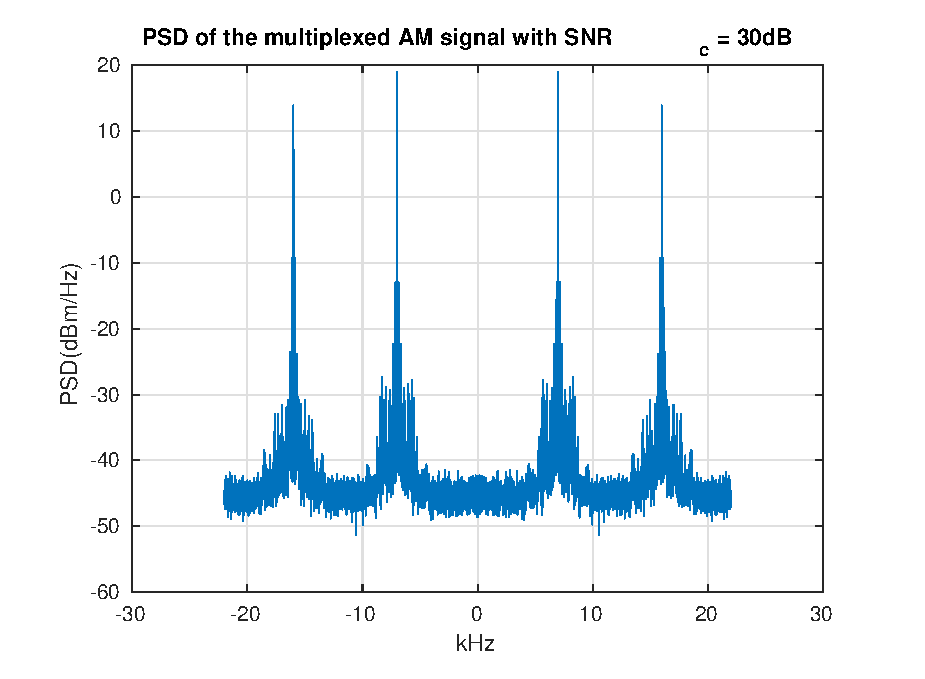
\includegraphics{imagens/multiplexed_30db.eps}
	\caption{$\hat{x}$ at a $SNR_c$ of 30 db}
	\label{fig:multi_30}
\end{figure}

The resulting PSD of $\hat{x}$ At a $SNR_c$ of $-5$ dB is described in the Fig.~\ref{fig:multi_5}.

\begin{figure}[h!]
	\centering
	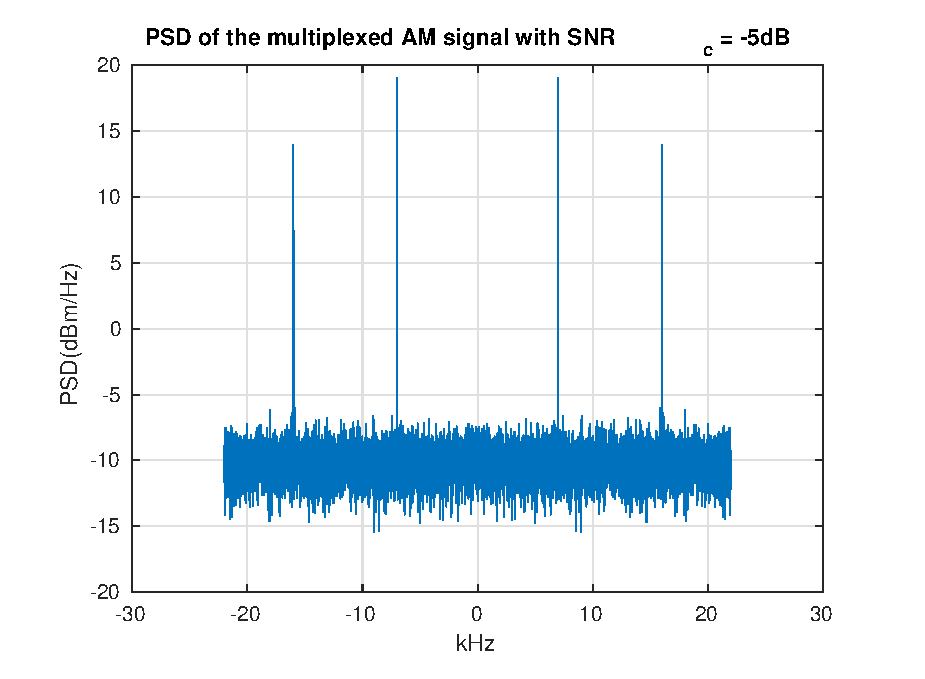
\includegraphics{imagens/multiplexed_5db.eps}
	\caption{$\hat{x}$ at a $SNR_c$ of -5 db}
	\label{fig:multi_5}
\end{figure}

After trasmitting $\hat{x}$ over the AWGN channel, the task objective consist in demultiplex the signal $\hat{x}$ and then demodulate and extract the information $\hat{x}_1$ and $\hat{x}_2$ that correspond directly to $x_1$ and $x_2$ respectively. To do so, the first step is a frequency downconversion as follows:

\begin{align}
	\hat{x}_{down}(t) &= \hat{x}(t)carrier(t) \\ \nonumber
	\hat{x}_{down}(t) &= \hat{x}(t)(e^{-j2\pi*Fc*t}).
\end{align}

Then the downconverted signal pass at suceptive fiters, to first eliminate the images from the negative frequency shifted to the positive frequency. The second filter eliminates the component of the other carrier, and the last filter isolates the information signal. The Figs. \ref{fig:hat_x1} and \ref{fig:hat_x2} show the result of this process to $\hat{x}_1$ and $\hat{x}_2$ respectively.
\begin{figure}[h!]
	\centering
	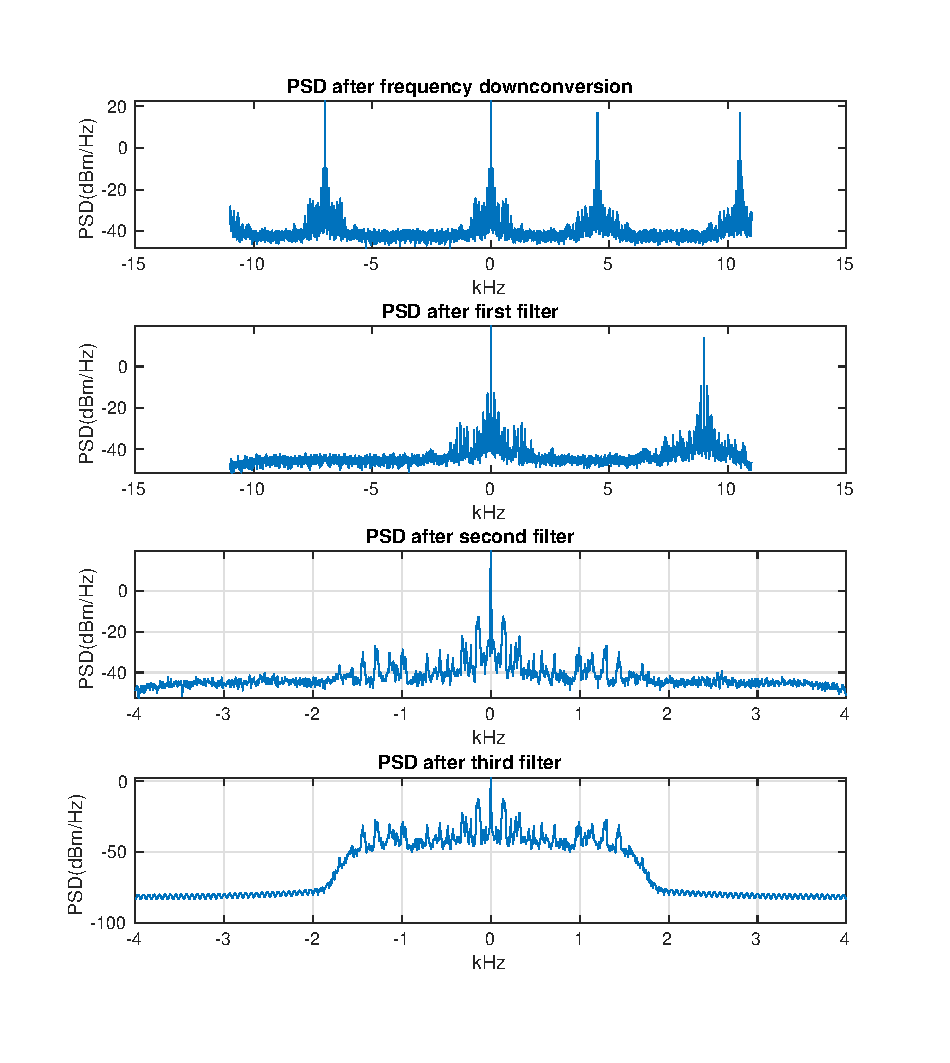
\includegraphics{imagens/x1hat.eps}
	\caption{$\hat{x}_1$ at a $SNR_c$ of 30 db}
	\label{fig:hat_x1}
\end{figure}

\begin{figure}[h!]
	\centering
	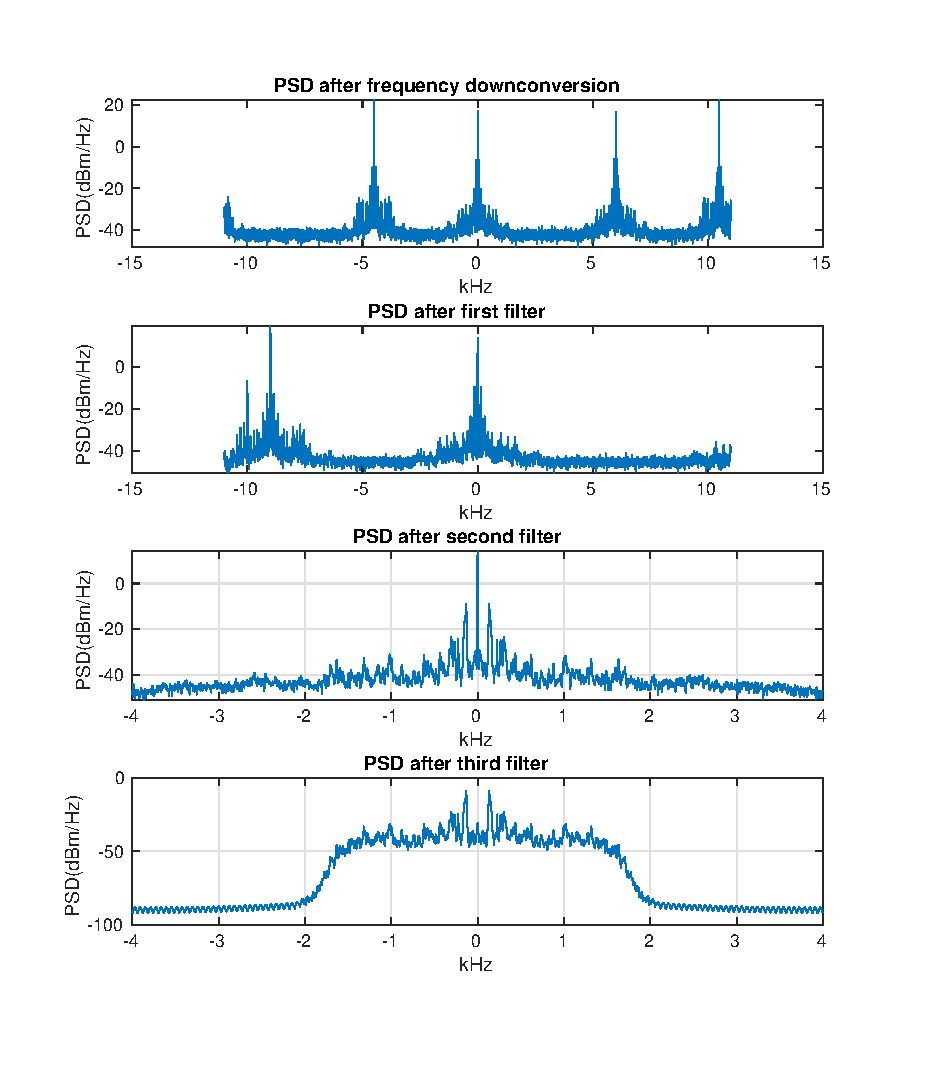
\includegraphics{imagens/x2hat.eps}
	\caption{$\hat{x}_2$ at a $SNR_c$ of 30 db}
	\label{fig:hat_x2}
\end{figure}

After this process, it was possible to trace a relationship between $SNR_c$ and $SNR_d$, using different white noise power levels. This relation is ilustrated in the Fig.~\ref{fig:snr}

\begin{figure}[h!]
	\centering
	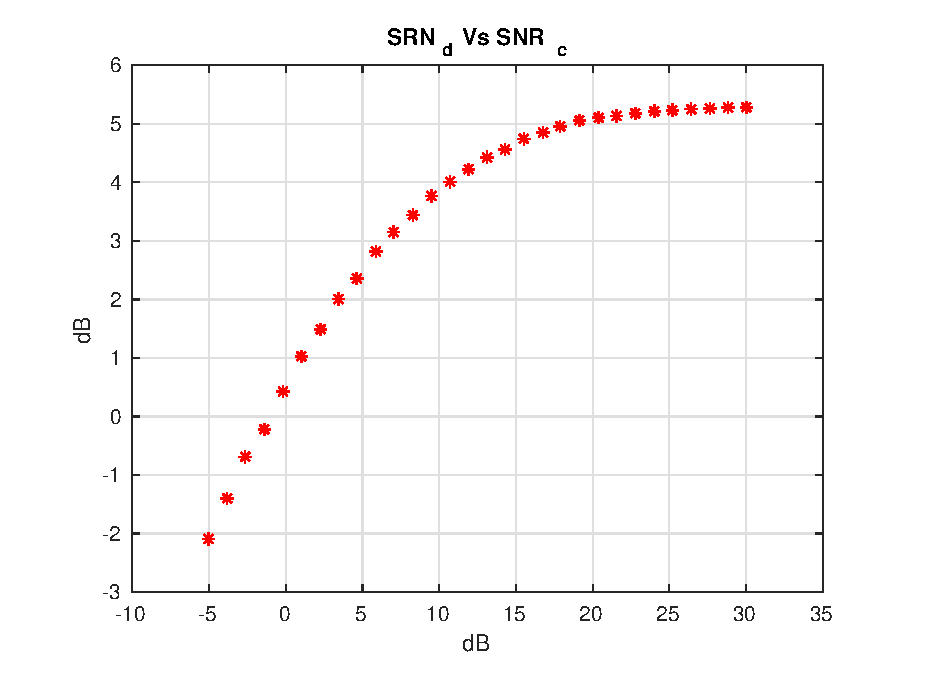
\includegraphics{imagens/SNR.eps}
	\caption{$SNR_c$ and $SNR_d$ relation}
	\label{fig:snr}
\end{figure}

% ----------------------------------------------------------
% ELEMENTOS PÓS-TEXTUAIS
% ---------------------------------------------------------


\end{document}
